\documentclass[10pt]{article}
\usepackage[utf8]{inputenc}
\usepackage[activeacute,spanish]{babel}
\usepackage[left=1.5cm,top=1.5cm,right=1.5cm, bottom=1.5cm,letterpaper, includeheadfoot]{geometry}

\usepackage{amssymb, amsmath, amsthm}
\usepackage{graphicx}
\usepackage{hyperref}
\usepackage{lmodern,url}
\usepackage{paralist} %util para listas compactas
\usepackage{xcolor}
\usepackage{bbm}
\usepackage{mathrsfs}
\usepackage{bbm}

%========PAQUETES AGREGADOS===========
%Pseudocodigo
\usepackage{pseudocode}
\usepackage[portuguese, boxruled]{algorithm2e}
\usepackage{wrapfig}
\usepackage{multicol}
\usepackage{graphicx}
\usepackage{caption}
\usepackage{subcaption}
%\captionsetup[table]{labelformat=empty}
\captionsetup[subfigure]{labelformat=empty}
\usepackage{cancel}
\usepackage{tikz}
\def\checkmark{\tikz\fill[scale=0.4](0,.35) -- (.25,0) -- (1,.7) -- (.25,.15) -- cycle;} 
%====================================

\usepackage{fancyhdr}
\pagestyle{fancy}
\fancypagestyle{plain}{%
\fancyhf{}
\lhead{\footnotesize\itshape\bfseries\rightmark}
\rhead{\footnotesize\itshape\bfseries\leftmark}
}


% macros
\newcommand{\Q}{\mathbb Q}
\newcommand{\R}{\mathbb R}
\newcommand{\N}{\mathbb N}
\newcommand{\Z}{\mathbb Z}
\newcommand{\C}{\mathbb C}
\newcommand{\BigO}{\mathcal{O}}
%Teoremas, Lemas, etc.
\theoremstyle{plain}
\newtheorem{teo}{Teorema}
\newtheorem{lem}{Lema}
\newtheorem{prop}{Proposición}
\newtheorem{cor}{Corolario}
\newtheorem{obs}{Observación}
\newtheorem{ej}{Ejemplo}
\renewcommand{\qedsymbol}{\rule{0.7em}{0.7em}}
\renewenvironment{proof}{{\bfseries \noindent Demostración}}{ \qed \\}


\theoremstyle{definition}
\newtheorem{defi}{Definición}
% fin macros


\newcommand{\catnum}{11} %numero de catedra
\newcommand{\fecha}{13 de Septiembre 2016 }

%%%%%%%%%%%%%%%%%%

%Macros para este documento
\newcommand{\cin}{\operatorname{cint}}



\begin{document}
%Encabezado
\fancyhead[L]{Facultad de Ciencias Físicas y Matemáticas}
\fancyhead[R]{Universidad de Chile}
\vspace*{-1.2 cm}
\begin{minipage}{0.6\textwidth}
\begin{flushleft}
\hspace*{-0.5cm}\textbf{MA3402-1 Estadística. Primavera 2016}\\
\hspace*{-0.5cm}\textbf{Profesor:} Raul Gouet\\
\hspace*{-0.5cm}\textbf{Escriba:} Manuel Cáceres\\
\hspace*{-0.5cm}\textbf{Fecha:} \fecha
\end{flushleft}
\end{minipage}
\begin{minipage}{0.36\textwidth}
\begin{flushright}

\includegraphics[scale=0.3]{imagenes/fcfm_dcc}
\end{flushright}
\end{minipage}
\bigskip
%Fin encabezado

\begin{center}
\LARGE\textbf{Clase \catnum}
\end{center}
Recuerdo del problema bilateral $X_{1},\ldots,X_{n} \sim N(\mu,\sigma^2), \sigma$ conocido, $H_{0}: \mu=\mu_{0}$ versus $H_{1}: \mu \not = \mu_{0}$ (bilateral).\\

Los tests clasicos de NP para $H_{0}: \mu=\mu_{0}$ versus $H_{1}: \mu=\mu_{1}, \mu_{1}>\mu_{0}$ o $H_{0}: \mu=\mu_{0}$ versus $H_{1}: \mu_{1}<\mu_{0}$ no sirven para el problema bilateral, en realidad no son UMP (y por mucho).\\

Test a la derecha (1) $\bar{X} \ge \mu_{0} + \frac{\sigma}{\sqrt{n}}\phi^{-1}(1-\alpha)$ y a la izquierda (2) $\bar{X} \ge \mu_{0} + \frac{\sigma}{\sqrt{n}}\phi^{-1}(\alpha)$.\\

Estrategia de la micro para el problema bilateral: Duplicar el test NP.\\

Rechazamos $H_{0}:\mu=\mu_{0}$ en lugar de $H_{1}:\mu \not \mu_{0}$ si alguno de los TNP rechaza, i.e. tiene función $max\{\phi_{1}(X),\phi_{2}(X)\}$.\\

Veamos que
\begin{align*}
\phi(X) = 1 \Leftrightarrow & \bar{X} \ge \mu_{0} + \frac{\sigma}{\sqrt{n}}\phi^{-1}(1-\alpha) \lor \bar{X} \le \mu_{0} + \frac{\sigma}{\sqrt{n}}\phi^{-1}(\alpha)\\
\Leftrightarrow & \bar{X} \not \in [\mu_{0} + \frac{\sigma}{\sqrt{n}}\phi^{-1}(\alpha), \mu_{0} + \frac{\sigma}{\sqrt{n}}\phi^{-1}(1-\alpha)]
\end{align*}
\begin{center}
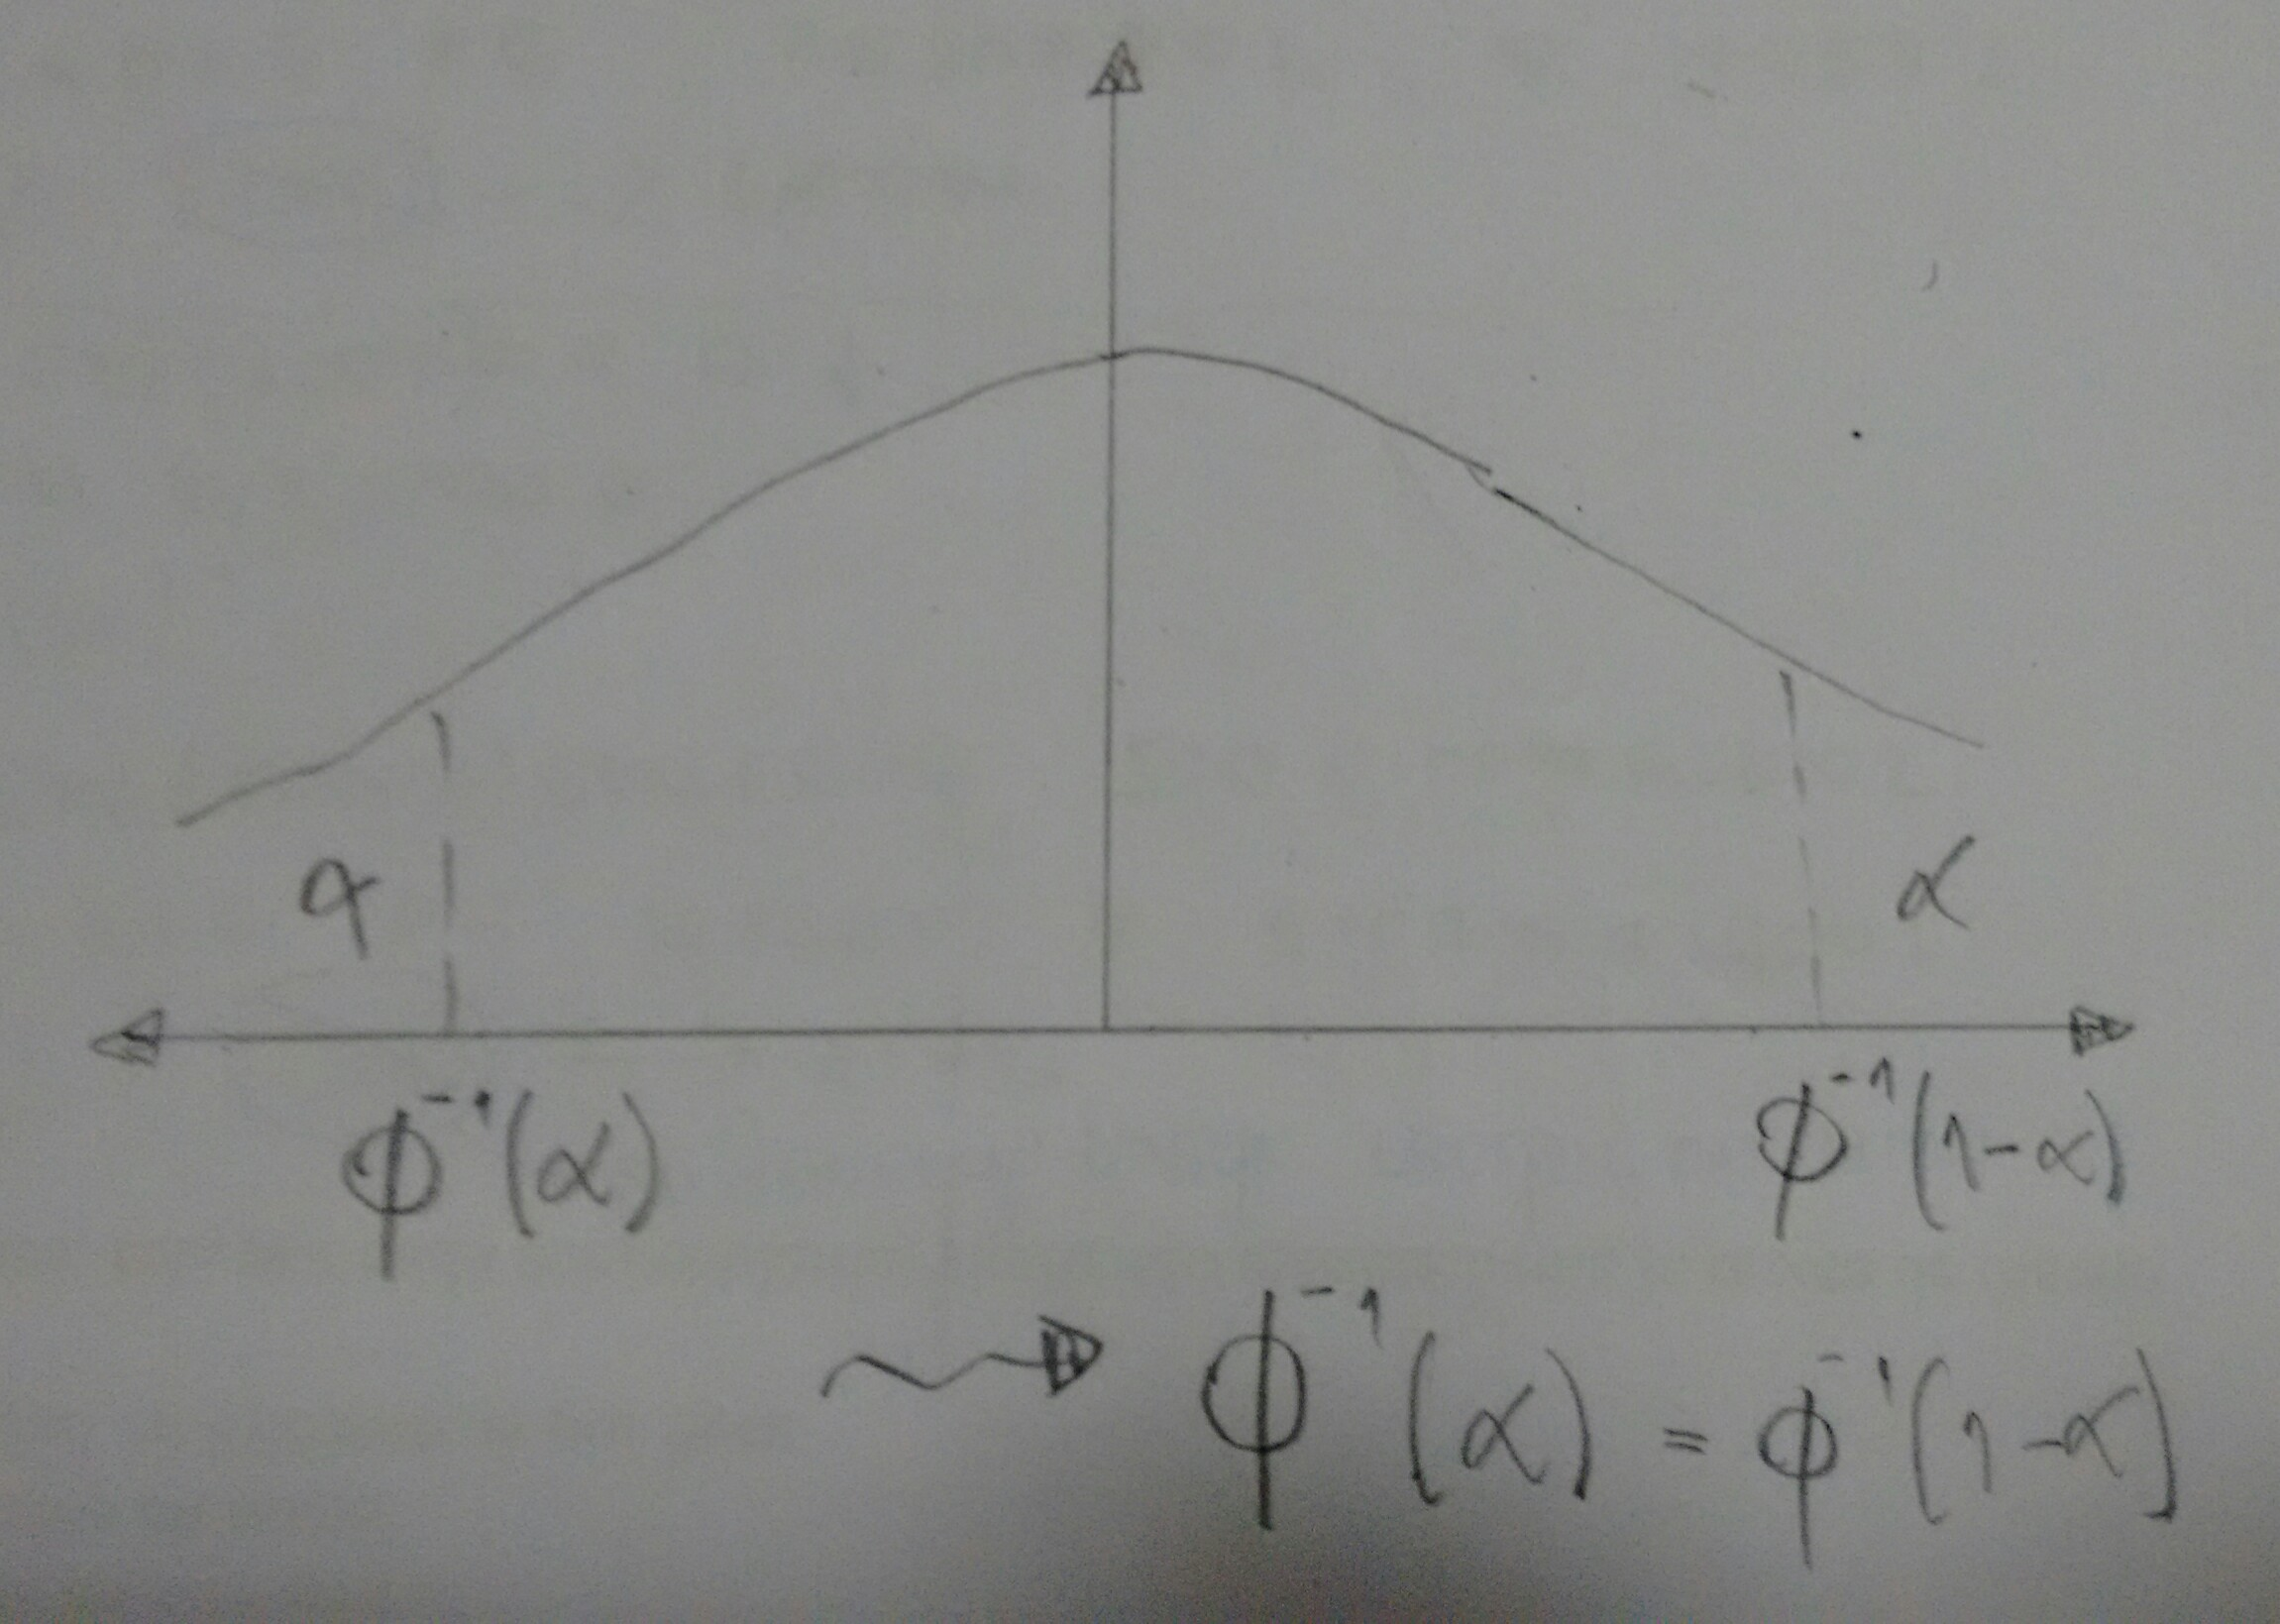
\includegraphics[scale=0.1]{imagenes/micro.jpg}
\end{center}
\begin{align*}
\mathbb{P}_{\mu_{0}}(\phi(X)=1)&\\
&= \mathbb{P}_{\mu_{0}}(\bar{X}\not \in [\ldots])\\
&= \mathbb{P}_{\mu_{0}}\left(\frac{|\bar{X}-\mu_{0}|}{\sigma/\sqrt{n}}>\phi^{-1}(1-\alpha)\right)\\
&= 2\alpha
\end{align*}
que es el mismo test que rechaza cuando $|\bar{X}-\mu_{0}|$ es grande.

\section{Ejercicios del TRV}
Recordemos que el TRV para $H_{0}: \theta \in \Theta_{0}$ versus $H_{1}: \theta \in \Theta_{1}$ tiene región crítica $\mathbb{R}=\{X \colon \lambda(X) \ge k_{\alpha}\}$ y tal que $\sup_{\Theta_{0}}\mathbb{P}_{\theta}(\lambda(X) \ge k_{\alpha})\le \alpha$, con 
\begin{align*}
\lambda(X) &= \frac{\sup_{\theta \in \Theta_{1}}f_{\theta}(X)}{\sup_{\theta \in \Theta_{0}}f_{\theta}(X)}\\
&= \frac{f_{\hat{\theta_{1}}}}{f_{\hat{\theta_{0}}}}
\end{align*}
que son EMV de $\theta$ restringidos a $\Theta_{0} y \Theta_{1}$.\\
\textbf{Minitruco útil en ocasiones}\\

Sea
\begin{align*}
\tilde{\lambda}(X) &= \frac{\sup_{\theta \in \Theta}f_{\theta}(X)}{\sup_{\theta \in \Theta_{0}}f_{\theta}(X)}\\
&= \frac{\max\{\sup_{\theta \in \Theta_{0}}f_{\theta}(X),\sup_{\theta \in \Theta_{1}}f_{\theta}(X)\}}{\sup_{\theta \in \Theta_{0}}f_{\theta}(X)}\\
&= \max\{1,\lambda(X)\}
\end{align*}
Veamos que $\tilde{\lambda}$ es función creciente de $\lambda$ y $\lambda(X) \ge k_{\alpha} \Leftrightarrow \tilde{\lambda}(X) \ge k_{\alpha}'$.\\
El TRV se puede trabajar según $\lambda$ o $\tilde{\lambda}$ según convenga.\\

Veamos un ejemplo:\\
$X_{1},\ldots,X_{n}$ iid $N(\mu,\sigma^2)$ y tenemos $H_{0}: \mu=\mu_{0}$ versus $H_{1}: \mu > \mu_{0}$, $\Theta_{0}=\{\mu_{0}\}$ , $\Theta_{1}=(\mu_{0},\infty)$, $\Theta = [\mu_{0},\infty)$
\begin{align*}
\lambda(X) &= \frac{\sup_{\Theta_{1}}f_{\mu}(X)}{\sup_{\Theta_{0}}f_{\mu}(X)}\\
&= \frac{\sup_{\mu>\mu_{0}}f_{\mu}(X)}{\sup_{\mu =\mu_{0}}f_{\mu}(X)}\\
&= \frac{\sup_{\mu>\mu_{0}}f_{\mu}(X)}{\sup_{\mu_{0}}f_{\mu}(X)}\\
&= \sup_{\mu > \mu_{0}} k e^{-\frac{1}{2\sigma^2}\sum(X_{i}-\mu)^2}
\end{align*}
Que es equivalente al problema
\begin{align*}
\min_{\mu>\mu_{0}} \underbrace{\sum(X_{i}-\mu)^2}_{g(\mu)}
\end{align*}
$g$ es función convexa de $\mu$ en $\mathbb{R}$ y tiene mínimo global que resulta ser $\bar{X}$.\\

\begin{itemize}
\item Si $\bar{X} \in (\mu_{0},\infty)$, entonces $\hat{\mu_{0}} = \bar{X}$
\item Si $\bar{X}\le \mu_{0}$, entonces $\hat{\mu_{0}}=\mu_{0}$
\end{itemize}
Luego $\hat{\mu_{0}} = \bar{X}\mathbbm{1}_{\{\bar{X}>\mu_{0}\}}+ \mu_{0} \mathbbm{1}_{\bar{X}\le \mu_{0}}$ 
\begin{align*}
\Rightarrow &\lambda(X) = e^{-\frac{1}{2\sigma^2}\left(\sum (X_{i}-\hat{\mu_{0}})^2- \sum (X_{i}-\mu_{0})^2\right)}\ge k_{\alpha}\\
\Leftrightarrow & \sum (X_{i}-\mu_{0})^2 - \sum (X_{i}-\hat{\mu_{0}})^2 \ge k_{\alpha}'\\
\Leftrightarrow &-2n\mu_{0} + n\mu_{0}^2 +2n\bar{X}\hat{\mu_{0}} - n \hat{\mu_{0}}^2 \ge k_{\alpha}'\\
\Leftrightarrow &2\bar{X}(\hat{\mu_{0}}-\mu_{0}) - (\hat{\mu_{0}})^2-\mu_{0}^2) \ge k_{\alpha}''
\end{align*}
Pero $\hat{\mu_{0}} - \mu_{0} = \bar{X}\mathbbm{1}_{\bar{X}>\mu_{0}} + \mu_{0}\mathbbm{1}_{\bar{X}\le \mu_{0}} - \mu_{0}\mathbbm{1}_{\bar{X}>\mu_{0}} - \mu_{0}\mathbbm{1}_{\bar{X}\le \mu_{0}} = (\bar{X}-\mu_{0})\mathbbm{1}_{\bar{X}\le \mu_{0}}$
\begin{align*}
\Leftrightarrow & 2\bar{X}(\bar{X}-\mu_{0})\mathbbm{1}_{\bar{X}>\mu_{0}} - (\bar{X}^2-\mu_{0}^2)\mathbbm{1}_{\bar{X}>\mu_{0}} \ge k_{\alpha}''
\end{align*}
por la definición de $\hat{\mu_{0}}$ (viendo indicatrices) se tiene que $\hat{\mu_{0}}^2 = \bar{X}^2 + \mu_{0}^2$
\begin{align*}
&(\bar{X}-\mu_{0})\mathbbm{1}_{\bar{X}>\hat{\mu_{0}}}(2\bar{X}- (\bar{X}+\mu_{0})) = (\bar{X}-\mu_{0})^2\mathbbm{1}_{\bar{X>\hat{\mu_{1}}}}\\
\Leftrightarrow \bar{X}-\mu_{0} \ge k_{\alpha}'''
\end{align*}
Esta última constante la calculamos $\mathbb{P}_{\mu_{0}}\left(\frac{\bar{X}-\mu_{0}}{\sigma/\sqrt{n}}>\frac{k_{\alpha}'''}{\sigma/\sqrt{n}}\right)= \alpha$\\

¿Qué ocurre si $\sigma$ es desconocido?\\

$H_{0}:\mu=\mu_{0}$ versus $H_{1}: \mu > \mu_{0}$, $\theta = (\mu,\sigma)$, $\Theta_{0}=\{\mu_{0}\}\times (0,\infty)$ y $\Theta_{1}=(\mu_{0},\infty)\times (0,\infty)$.
\begin{align*}
&\lambda(X) = \frac{\sup_{\sigma>0}\sup_{\mu>\mu_{0}}f_{\theta}(X)}{\sup_{\sigma>0}\sup_{\mu=\mu_{0}}f_{\theta}(X)}\\
\sup_{\sigma>0}\sup_{\mu=\mu_{0}}f_{\theta}(X) &= \sup_{\sigma>0} \left(\frac{1}{\sqrt{2\pi}}\right)^n\sigma^{-n}e^{-1/2\sigma^2}\sum (X_{i}-\mu_{0})^2\\
\Leftrightarrow &\max_{\sigma>0} -n\log \left(-\frac{1}{2\sigma^2}\sum (X_{i}-\mu_{0})^2\right)\\
\Rightarrow & \hat{\sigma_{0}} = \frac{1}{n} \sum (X_{i}-\mu_{0})^2
\end{align*}
\begin{itemize}
\item $\sup_{\mu>\mu_{0}}k\sigma^{-n}e^{-\frac{1}{2\sigma^2}\sum (X_{i}- \mu)^2} = k \sigma^{-n}e^{-\frac{1}{2\sigma^2}\sum (X_{i}-\hat{\mu_{0}})^2}$
\item $\sup_{\sigma>0}k\sigma^{-n}e^{-\frac{1}{2\sigma^2}\sum (X_{i}- \hat{\mu_{0}})^2} = k \hat{\sigma_{1}}^{-n}e^{-\frac{1}{2\hat{\sigma_{1}}^2}\sum (X_{i}-\hat{\mu_{0}})^2}$
\item Por lo tanto, $\hat{\sigma_{1}} = \frac{1}{n}\sum (X_{i}-\hat{\mu_{0}})^2$
\end{itemize}
\begin{align*}
\Rightarrow & \frac{\hat{\sigma_{0}}^{-n}e^{-\frac{1}{2\hat{\sigma_{0}}}\sum (X_{i}-\mu_{0})^2}}{\hat{\sigma_{1}}^{-n}e^{-\frac{1}{2\hat{\sigma_{1}}}\sum (X_{i}-\hat{\mu_{1}})^2}} = \left(\frac{\hat{\sigma_{1}}^2}{\hat{\sigma_{0}}^2}\right)^{n/2}\\
\Leftrightarrow & \lambda(X) \ge k_{\alpha} ssi \frac{\hat{\sigma_{1}}^2}{\hat{\sigma_{0}}^2} \ge k_{\alpha}'\\
\Leftrightarrow &\frac{n\sigma^2 + n(\bar{X}-\hat{\mu_{1}})^2}{n\sigma^2+n(\bar{X}-\mu_{0})^2}\ge k_{\alpha}'\\
\Leftrightarrow &\frac{1 + \left(\frac{\bar{X}-\hat{\mu_{1}}}{\hat{\sigma}}\right)^2}{1 + \left(\frac{\bar{X}-\mu_{0}}{\hat{\sigma}}\right)^2}\ge k_{\alpha}''\\
\end{align*}
Con un nikita-nipone obtenemos que $\bar{X}-\hat{\mu_{1}} = (\bar{X}-\mu_{0})\mathbbm{1}_{\bar{X}\le \mu_{0}}$. Desarrollando lo anterior llegamos a la función $\frac{1+y^2}{1+y^2\mathbbm{1}_{y\le0}}$ que es una función creciente de $\frac{\bar{X}-\mu_{1}}{\hat{\sigma}^2}$ que es una t de student.
\end{document}